\documentclass[11pt,onecolumn]{article}

\usepackage[margin=0.95in,top=0.85in,bottom=0.85in]{geometry}
\usepackage{amsmath,amssymb}
\usepackage{graphicx}
\usepackage{booktabs}
\usepackage[hidelinks,unicode=false]{hyperref}
\pdfstringdefDisableCommands{%
  \let\c\relax \let\i\relax
}
\usepackage[protrusion=true,expansion=false]{microtype}
\usepackage{parskip}
\usepackage{caption}
\usepackage[numbers,sort&compress]{natbib}
\usepackage[compact]{titlesec}
\titlespacing*{\section}{0pt}{6pt plus 2pt minus 1pt}{3pt plus 1pt}
\titlespacing*{\subsection}{0pt}{5pt plus 2pt minus 1pt}{2pt plus 1pt}
\titlespacing*{\paragraph}{0pt}{4pt plus 1pt minus 1pt}{0.5em}

% Tighter float and paragraph spacing
\setlength{\floatsep}{4pt plus 1pt minus 1pt}
\setlength{\textfloatsep}{6pt plus 2pt minus 2pt}
\setlength{\intextsep}{4pt plus 1pt minus 1pt}
\setlength{\parskip}{2pt plus 1pt}
\setlength{\abovecaptionskip}{4pt}
\setlength{\belowcaptionskip}{0pt}

\graphicspath{{figures/}}

% Convenience macros
\newcommand{\dmin}{d_{\min}}
\newcommand{\Rbb}{\mathbb{R}}

\title{\textbf{Comparing Consensus ADMM and Penalty Methods for\\
Distributed Multi-Agent Trajectory Planning}}

\author{Christian Yu \quad Yuyang Wu \quad Yen-Ru Chin \\[0.3em]
\small Department of Electrical and Computer Engineering \\
\small Carnegie Mellon University \\
\small \texttt{\{cjyu, yuyangw2, yenruc\}@andrew.cmu.edu}}

\date{}

\begin{document}

\maketitle
\thispagestyle{empty}

%% ---------------------------------------------------------------
\section{Introduction}
\label{sec:intro}
%% ---------------------------------------------------------------

Distributed optimization is central to coordinating cyber-physical systems (CPS), where
agents must cooperatively solve a global objective through local computation and neighbor
communication \cite{notarstefano2019}.  A canonical example is multi-drone
trajectory planning: each drone must navigate to its own goal while avoiding collisions with
nearby agents, without a central coordinator that has access to all agents' states simultaneously.

Two main classes of distributed methods handle the inter-agent collision constraint
differently.  The \emph{penalty method} incorporates constraint violations directly into each agent’s local objective via a quadratic penalty term, requiring only trajectory broadcast among neighboring agents.  It is relatively simple to implement, but its effectiveness hinges entirely on the choice of a scalar penalty weight $w$: if $w$ is too small, collisions may occur; if too large, the resulting per-agent QP becomes ill-conditioned and can even lead to \emph{increased} constraint violations.
The \emph{Alternating Direction Method of Multipliers (ADMM)} augments the penalty with
dual variables that iteratively enforce feasibility \cite{boyd2011admm}.
The \emph{Consensus} variant of ADMM, designed for graph-structured multi-agent systems \cite{chen2024tutorial}, maintains pairwise dual variables $\lambda_{ij}$
that accumulate consensus errors and enforce the separation constraint asymptotically,
independent of any single scalar knob.

This report compares penalty and Consensus ADMM on multi-drone trajectory planning with
collision avoidance, using a centralized joint QP as the optimal reference.  For each
method we derive predictions about its expected parameter sensitivity from first principles and
validate them against parameter sweeps in simulation.  Three questions guide the
investigation: (1) Do both methods converge to the centralized optimum?  (2) How
sensitive is each method to its tuning parameter ($w$ for penalty, $\rho$ for ADMM)?
(3) How does each method scale with respect to the number of drones $N$?

%% ---------------------------------------------------------------
\section{Background and Motivation}
\label{sec:background}
%% ---------------------------------------------------------------

\paragraph{Model Predictive Control (MPC).}
At each time step $t$, MPC solves a finite-horizon optimal control problem from the current
state, applies only the first control action, advances the state, and repeats.  This
receding-horizon structure tolerates linearization errors in the far horizon because they
are corrected at the next re-solve.  For multi-agent settings, MPC
naturally decomposes into per-agent subproblems coupled only through the collision constraints.

\paragraph{Double-integrator dynamics.}
Each drone is a 2D point mass with state
$x_i = [p_i^\top,\, v_i^\top]^\top \in \Rbb^4$ and control $u_i \in \Rbb^2$
(acceleration).  Zero-order-hold discretization at $\Delta t$ gives
$A = \bigl[\begin{smallmatrix} I & \Delta t I \\ 0 & I \end{smallmatrix}\bigr]$,
$B = \bigl[\begin{smallmatrix} \frac{1}{2}\Delta t^2 I \\ \Delta t I \end{smallmatrix}\bigr]$.
This model is standard in the DMPC literature \cite{luis2020online} and is justified by
quadrotor differential flatness \cite{mellinger2011}: a smooth position trajectory uniquely
determines the attitude and motor commands needed to track it, so the planner only needs
to reason about position.

\paragraph{Linearized collision avoidance.}
The safety constraint $\|p_i(k) - p_j(k)\|_2 \ge \dmin$ is nonconvex, so we handle it
via \emph{sequential convex programming} (SCP). 
At the current estimate $\bar{p}_i(k),\, \bar{p}_j(k)$, we form the unit normal
\[
  n_{ij}(k) = \frac{\bar p_i(k) - \bar p_j(k)}{\|\bar p_i(k) - \bar p_j(k)\|_2}
\]
and impose the linearized half-space $n_{ij}(k)^\top (p_i(k) - p_j(k)) \ge \dmin$.
Re-linearizing once per MPC time step keeps each agent's subproblem a convex QP.

%% ---------------------------------------------------------------
\section{Problem Formulation}
\label{sec:problem}
%% ---------------------------------------------------------------

We consider $N$ drones communicating over a graph $\mathcal{G} = (\mathcal{V}, \mathcal{E})$,
where $\mathcal{V} = \{1,\ldots,N\}$ indexes the drones and $(i,j) \in \mathcal{E}$ iff
drones $i$ and $j$ exchange planned trajectories.  We write
$\mathcal{N}_i = \{j : (i,j) \in \mathcal{E}\}$ for the neighbors of drone $i$; collision
constraints are enforced only between neighbors, since $i$ only has access to the
planned trajectory of $j$ when $j \in \mathcal{N}_i$.
Each drone $i$ solves the finite-horizon tracking problem
\begin{equation}
  \min_{\{x_i,\, u_i\}} \; \sum_{k=0}^{H} \|x_i(k) - x_i^{\mathrm{ref}}\|^2
                          + \sum_{k=0}^{H-1} \|u_i(k)\|^2
  \label{eq:per_agent}
\end{equation}
subject to dynamics $x_i(k+1) = A x_i(k) + B u_i(k)$, initial condition
$x_i(0) = x_i^{\mathrm{measured}}$, control bounds $\|u_i(k)\|_\infty \le u_{\max}$ (the quadrotor's acceleration limit),
and the linearized collision half-spaces for all $j \in \mathcal{N}_i$ and $k = 0,\ldots,H$.
The reference $x_i^{\mathrm{ref}}$ is the goal state (target position, zero velocity), so
the cost rewards reaching the goal and staying there.

The three methods studied are differentiated by how they enforce the coupling constraint.

%% ---------------------------------------------------------------
\section{Methods}
\label{sec:methods}
%% ---------------------------------------------------------------

\subsection{Centralized QP (Reference)}

The centralized reference combines all $N$ per-agent problems into a single joint QP:
\begin{equation}
  \min_{\{x_i, u_i\}_{i=1}^N} \; \sum_{i=1}^N \left(
    \sum_{k=0}^{H} \|x_i(k) - x_i^{\mathrm{ref}}\|^2
    + \sum_{k=0}^{H-1} \|u_i(k)\|^2 \right)
  \label{eq:centralized}
\end{equation}
subject to dynamics, bounds, and the linearized half-spaces for \emph{all} pairs
$(i,j) \in \mathcal{E}$.  The decision variable count scales as
$\mathcal{O}(N H)$ and the number of coupling constraints as $\mathcal{O}(|\mathcal{E}| H)$,
so the joint QP grows quadratically with $N$ on a dense graph.  We solve it with
CVXPY/OSQP \cite{stellato2020osqp}, wrapping it in a 5-iteration SCP loop that
re-linearizes the collision normals.

\subsection{Distributed Penalty Method}

Each drone adds a quadratic penalty for collision violations to its own objective and
iterates the following two steps until convergence:

\begin{enumerate}
  \item \textbf{Primal update.}  Drone $i$ solves
    \[
      \min_{x_i, u_i} \;
        \sum_{k=0}^{H}\!\bigl(\|x_i(k)-x_i^{\mathrm{ref}}\|^2
        + \|u_i(k)\|^2\bigr)
        + w \sum_{j \in \mathcal{N}_i} \sum_{k=0}^{H}
          \max\!\bigl(0,\; \dmin - n_{ij}(k)^\top(p_i(k)-p_j(k))\bigr)^2
    \]
    using the latest broadcast trajectories of its neighbors as fixed parameters.
  \item \textbf{Broadcast.}  Drone $i$ transmits its updated planned trajectory
    $\{x_i^{k+1}\}$ to all $j \in \mathcal{N}_i$.
\end{enumerate}

No dual variables are maintained; the only knob is the penalty weight $w$.

\subsection{Consensus ADMM}

\paragraph{Consensus reformulation.}
We lift each drone's decision variable to an \emph{augmented} local variable
$\Theta_i = (\theta_i,\, \{\tilde\theta_{ij}\}_{j \in \mathcal{N}_i})$, where
$\theta_i$ is the stacked trajectory $(x_i(0), u_i(0), \ldots, x_i(H))$ and
$\tilde\theta_{ij}$ is drone $i$'s local copy of neighbor $j$'s trajectory.
The inter-agent coupling is replaced by the consensus constraint
$\tilde\theta_{ij} = \theta_j$ for each edge $(i,j) \in \mathcal{E}$, and the
collision half-space uses $\tilde\theta_{ij}$ so the per-agent QP remains purely
local.

\paragraph{Augmented Lagrangian.}
Attaching a scaled dual variable $\lambda_{ij}$ to each directed consensus
constraint $\tilde\theta_{ij} = \theta_j$ gives the augmented Lagrangian
\cite{boyd2011admm,chen2024tutorial}:
\begin{equation}
  \mathcal{L}_\rho = \sum_{i \in \mathcal{V}} g_i(\Theta_i)
  + \sum_{i \in \mathcal{V}} \sum_{j \in \mathcal{N}_i} \!\left[
      \lambda_{ij}^\top \bigl(\tilde\theta_{ij} - \theta_j\bigr)
      + \tfrac{\rho}{2}\bigl\|\tilde\theta_{ij} - \theta_j\bigr\|_2^2
    \right],
  \label{eq:aug_lag}
\end{equation}
where $g_i(\Theta_i)$ packages everything that is local to drone $i$:
\begin{equation}
  g_i(\Theta_i) = \underbrace{\sum_{k=0}^{H} \|x_i(k) - x_i^{\mathrm{ref}}\|^2
                  + \sum_{k=0}^{H-1} \|u_i(k)\|^2}_{\text{tracking + control cost}}
                  \;+\; \mathcal{I}_{\mathcal{C}_i}(\Theta_i),
  \label{eq:gi}
\end{equation}
and $\mathcal{I}_{\mathcal{C}_i}$ is the $\{0, +\infty\}$ indicator of the feasible set
$\mathcal{C}_i$ defined by the dynamics $x_i(k+1) = A x_i(k) + B u_i(k)$, the initial
condition $x_i(0) = x_i^{\mathrm{measured}}$, the control bounds
$\|u_i(k)\|_\infty \le u_{\max}$, and the linearized collision half-spaces between drone
$i$'s own position and its local belief $\tilde\theta_{ij}$ for every
$j \in \mathcal{N}_i$.

\paragraph{Algorithm.}
The three-step iteration is:

\textbf{Step 1. Primal (parallel over agents).}  Each drone $i$ solves jointly for
its own trajectory and its beliefs about its neighbors:
\begin{equation}
  \Theta_i^{k+1} = \operatorname*{arg\,min}_{\Theta_i} \left(
    g_i(\Theta_i)
    + \sum_{j \in \mathcal{N}_i} \!\left[
        (\lambda_{ij}^k)^\top \tilde\theta_{ij}
        + \tfrac{\rho}{2}\bigl\|\tilde\theta_{ij} - \theta_j^k\bigr\|_2^2
      \right] \right).
  \label{eq:admm_primal}
\end{equation}
We write the components of the minimizer as
$\Theta_i^{k+1} = (\theta_i^{k+1},\, \{\tilde\theta_{ij}^{\,k+1}\}_{j \in \mathcal{N}_i})$.

\textbf{Step 2. Communicate.}  Each drone broadcasts its own $\theta_i^{k+1}$ to its
neighbors.

\textbf{Step 3. Dual update (parallel over directed edges).}
\begin{equation}
  \lambda_{ij}^{k+1} = \lambda_{ij}^k + \rho\, \bigl(\tilde\theta_{ij}^{\,k+1} - \theta_j^{k+1}\bigr).
  \label{eq:admm_dual}
\end{equation}

This pattern requires no central aggregation; all communication is local to the graph
edges.  Convergence is declared when the primal residual
$r^k = \|\tilde\theta_{ij}^{k} - \theta_j^k\|$ and the dual residual
$s^k = \rho\|\theta_j^k - \theta_j^{k-1}\|$ fall below tolerances
$\varepsilon^{\mathrm{pri}}$ and $\varepsilon^{\mathrm{dual}}$ \cite{boyd2011admm}.

\paragraph{Implementation notes.}
A soft slack on each collision half-space with weight $w_{\mathrm{coll}} = 10^7$
prevents infeasibility crashes during early iterations when linearizations may be
degenerate; this is a numerical safety valve and does not participate in the
feasibility-driving mechanism.  The per-agent QPs in ADMM and the penalty method are
solved with Clarabel \cite{goulart2024clarabel}; the centralized joint QP uses OSQP
\cite{stellato2020osqp}.

%% ---------------------------------------------------------------
\section{Predictions}
\label{sec:theory}
%% ---------------------------------------------------------------

\paragraph{Penalty: feasibility versus conditioning.}
The penalty method does not guarantee convergence to feasibility.  As $w \to \infty$
violation scales by $\mathcal{O}(1/w)$, but the per-agent Hessian condition number
grows proportionally to $w$, so the outer iteration's per-step progress shrinks and
the loop exhausts its iteration budget and terminates with non-negligible residual violations.
This leads to a characteristic U-shaped relationship between $w$ and constraint violation: when $w$ is small, collisions persist because the penalty is too weak; when $w$ is large, numerical ill-conditioning dominates and again prevents effective convergence; only an intermediate range of $w$ yields satisfactory performance, where constraint enforcement and numerical stability are balanced.

\paragraph{ADMM: dual variables decouple feasibility from conditioning.}
Boyd et al.\ \cite{boyd2011admm} shows that Consensus ADMM converges for any
$\rho > 0$ under convex local costs (which our setting satisfies); the role of
$\rho$ is therefore not to drive feasibility but to shape the convergence rate.  Concretely,
the dual update \eqref{eq:admm_dual} is an integrator: at a fixed point,
$\lambda_{ij}^{k+1} = \lambda_{ij}^k$ forces exact consensus
$\tilde\theta_{ij} = \theta_j$.  Collision avoidance is enforced through a two-step chain:
First, the hard half-space inside $g_i$ keeps drone $i$ safe relative to its belief
$\tilde\theta_{ij}$ at every iteration. Second, $\lambda_{ij}$ corrects the belief to match
the neighbor's true broadcast state. Together they yield true inter-agent separation in the
limit.  The dual variable $\lambda_{ij}$ thus drives the feasibility,
while $\rho$ enters only as a step-size for the dual update and a curvature term in
the per-agent QP. The two jobs are handled by two separate quantities, unlike the single
weight $w$ in the penalty method.  This indicates that ADMM should be much less
sensitive to $\rho$ than penalty is to $w$: the violation curve should stay near
zero across a wide range of $\rho$, even though iteration count required to converge may exhibit
a U-shape from rate sensitivity.

%% ---------------------------------------------------------------
\section{Experimental Setup}
\label{sec:setup}
%% ---------------------------------------------------------------

We evaluate on two scenarios that stress the collision-avoidance coupling at increasing
scale:

\textbf{S1. Four-drone ring ($N=4$).}  Four drones start at $90^\circ$ intervals on a
circle of radius 3\,m and swap to antipodal goals.  All four trajectories cross near the
origin.  The communication graph is a ring, so each drone enforces collision constraints
only with its two ring neighbors; the two diagonal pairs are unconstrained (they are
further apart and less prone to collision in this geometry).
Parameters: $H=25$, $\Delta t = 0.2\,\text{s}$, $u_{\max}=3\,\text{m/s}^2$,
$\dmin=0.5\,\text{m}$.  Penalty uses $w=10^3$; ADMM uses $\rho=5$.

\textbf{S2. Eight-drone complete graph ($N=8$).}  Eight drones start at
$45^\circ$ intervals on a circle of radius 3\,m and swap antipodally.  The communication
graph is complete: every pair of drones enforces a collision constraint.
Parameters: $H=30$, $\Delta t = 0.2\,\text{s}$, $u_{\max}=3\,\text{m/s}^2$,
$\dmin=0.5\,\text{m}$.  Penalty uses $w=2\times10^3$; ADMM uses $\rho=300$.
The straight-line warm-start is degenerate at $N=8$ (all drones pass the origin at the
same step), so ADMM is seeded with the penalty output to break symmetry; the centralized
solver uses the same seed.

For both scenarios we report: the number of outer iterations (primal broadcasts) to
convergence, the final objective $J^\star$, the minimum pairwise distance
$\min_{i<j,k}\|p_i(k)-p_j(k)\|_2$, and the constraint violation (maximum distance by
which any pairwise separation falls below $\dmin$).

The SCP outer loop converges to a local KKT point of the nonconvex collision-avoidance
problem \cite{mao2016scp}, not the global optimum. Antipodal swaps have multiple
local minima (clockwise vs.\ counterclockwise orbits).  ``Centralized'' in this
report therefore refers to the local optimum reached by SCP from the shared seed
above, not the global optimum of the original problem.  All three methods optimize
against the same linearized collision constraints from the same seed, so the
comparison isolates the effect of the solver rather than the constraint model.

We record violation and iteration count for two sensitivity sweeps on S1: penalty over
$w \in [10^2, 10^4]$ and ADMM over $\rho \in [10^{-1}, 10^3]$, with eight and nine
log-spaced values respectively.  Both use a 10{,}000-iteration outer-loop cap.

%% ---------------------------------------------------------------
\section{Numerical Results}
\label{sec:results}
%% ---------------------------------------------------------------

\subsection{S1: Four-Drone Ring}

Figure~\ref{fig:S1} shows the planned trajectories for S1.  All three methods produce
visually smooth paths that reach the goal positions, and the three objective values agree
to within 0.04\%.  The critical distinction emerges in the constraint column of
Table~\ref{tab:S1}: the penalty method's minimum pairwise distance is $0.483\,\text{m}$,
which is $17\,\text{mm}$ inside the exclusion disk.  This is a real violation: it occurs
at a discrete MPC step where two drones are geometrically inside each other's safety
radius.  ADMM and the centralized solver both respect the $0.5\,\text{m}$ boundary to
solver tolerance.  In terms of iteration count, ADMM converges in 44 outer rounds versus
99 for penalty, reflecting the additional feedback from the dual variables.

\begin{figure}[h]
  \centering
  \includegraphics[width=0.92\linewidth]{fig_S2_trajectories.pdf}
  \caption{S1 ($N=4$, ring graph): planned trajectories from penalty (left),
  Consensus ADMM (center), and centralized (right).  Filled squares are start positions;
  hollow stars are goals.  All three reach their goals, but penalty's minimum pairwise
  distance falls $17\,\text{mm}$ below the safety threshold.}
  \label{fig:S1}
\end{figure}

\begin{table}[h]
  \centering
  \caption{S1 ($N=4$, ring graph) results.  Violation is
  $\max_{i<j,k}\,\max(0,\, \dmin - \|p_i(k)-p_j(k)\|_2)$.}
  \label{tab:S1}
  \begin{tabular}{@{}lcccc@{}}
    \toprule
    Method & Iterations & $J^\star$ & Min.\ dist.\ (m) & Violation (m) \\
    \midrule
    Penalty ($w=10^3$)   & 99  & 8944.8 & 0.483 & $1.67\times10^{-2}$ \\
    ADMM ($\rho=5$)      & 44  & 8948.6 & 0.517 & $0$ \\
    Centralized          & 5   & 8946.5 & 0.500 & $0$ \\
    \bottomrule
  \end{tabular}
\end{table}

\subsection{Penalty Sensitivity to $w$}

Figure~\ref{fig:sensitivity} sweeps $w$ over more than two decades.  Violation
shows the predicted U-shape: at small $w$ the collision cost is too weak to deter
overlap (${\sim}0.42\,\text{m}$ at $w=10^2$); at large $w$ the per-agent Hessian
becomes ill-conditioned and the outer iteration stalls, leaving violation at
${\sim}0.24\,\text{m}$ for $w=10^4$.  Both failure modes are visible in the
iteration panel: the iteration count climbs sharply at large $w$ as the
ill-conditioned QP slows convergence.  The sweet spot is narrow, and a single
decade in either direction substantially degrades feasibility.

\begin{figure}[h]
  \centering
  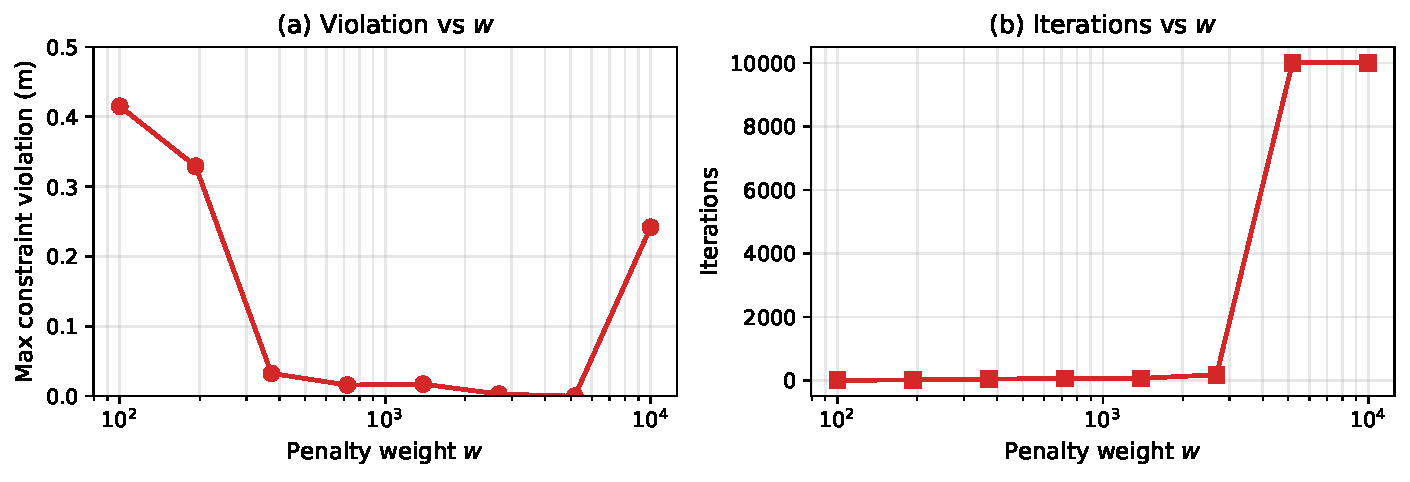
\includegraphics[width=0.92\linewidth]{fig_w_sensitivity.pdf}
  \caption{Penalty method sensitivity to $w$ on S1.  Left: constraint violation
  versus $w$.  Right: iteration count versus $w$.  The U-shape in violation
  reflects the fundamental tension between softness (left tail) and
  ill-conditioning (right tail).}
  \label{fig:sensitivity}
\end{figure}

\subsection{ADMM Sensitivity to $\rho$}

Figure~\ref{fig:rho_sensitivity} repeats the sweep for ADMM, sweeping $\rho$ over
four decades on the same scenario and the same $y$-axis.  The contrast with
penalty is stark: violation stays near zero across the entire range, with only
a small ${\sim}0.017\,\text{m}$ floor at $\rho \le 3$.  ADMM does exhibit a
U-shape in iteration count -- $\rho$ is a rate-control parameter, and convergence
slows at both extremes -- but the rate sensitivity does not translate into a
violation penalty: across nearly four decades of $\rho$ the algorithm achieves
true feasibility, validating the prediction that the dual variable carries the
feasibility-driving role separately from $\rho$.

\begin{figure}[h]
  \centering
  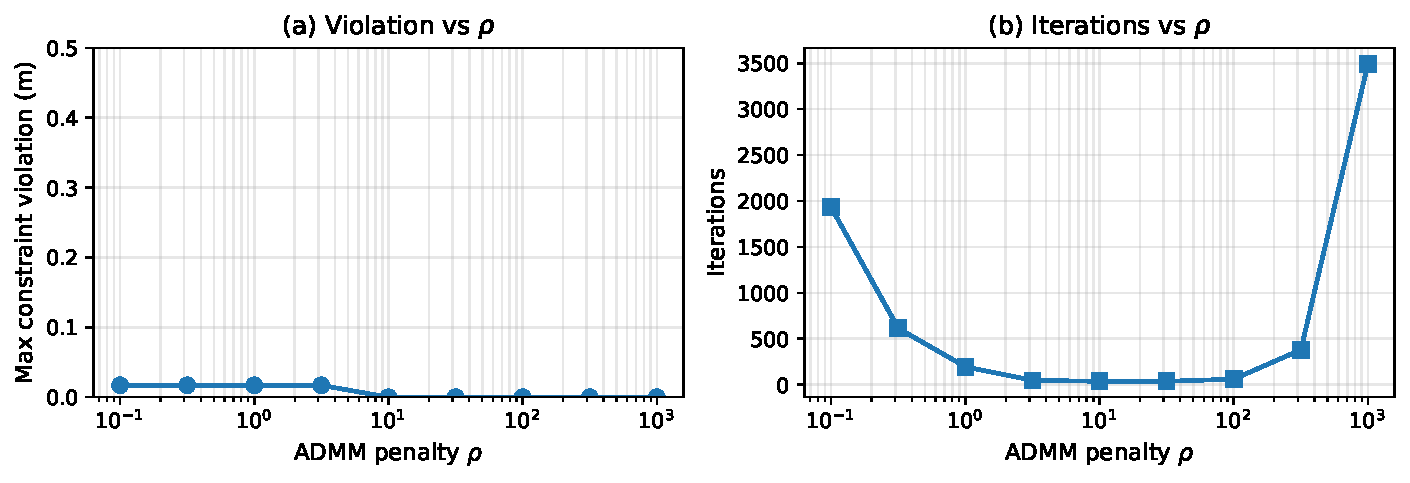
\includegraphics[width=0.92\linewidth]{fig_rho_sensitivity.pdf}
  \caption{ADMM sensitivity to $\rho$ on S1 (same $y$-axis as
  Figure~\ref{fig:sensitivity}).  Left: violation stays near zero across four
  decades of $\rho$, with a small floor at $\rho \le 3$.  Right: iteration count
  is U-shaped, reflecting $\rho$'s role as a rate parameter rather than a
  feasibility knob.}
  \label{fig:rho_sensitivity}
\end{figure}

\subsection{S2: Eight-Drone Complete Graph}

Figure~\ref{fig:S2} shows S2 trajectories.  The feasibility gap between penalty
and ADMM grows dramatically at $N=8$.  Penalty ($w=2\times10^3$) leaves a minimum
pairwise distance of $0.175\,\text{m}$, a violation of $0.325\,\text{m}$, roughly
$20\times$ larger than the S1 violation at a comparable $w$.
ADMM with $\rho=300$ matches the centralized objective to $0.03\%$ and achieves a
minimum distance of exactly $0.500\,\text{m}$, with residual violation below
$10^{-4}\,\text{m}$ (solver tolerance).  Table~\ref{tab:S2} summarizes the numbers.

The larger $\rho$ required at $N=8$ (300 vs.\ 5 at $N=4$) is consistent with theory:
each agent has 7 neighbors in the complete graph versus 2 in the ring, so the
consensus penalty term in \eqref{eq:aug_lag} has more terms.  A larger $\rho$ is needed
to maintain the same per-iteration dual feedback magnitude per constraint.

\begin{figure}[h]
  \centering
  \includegraphics[width=0.92\linewidth]{fig_S3_trajectories.pdf}
  \caption{S2 ($N=8$, complete graph): planned trajectories from penalty (left),
  Consensus ADMM (center), and centralized (right).  Penalty drones overlap by
  up to $0.33\,\text{m}$; ADMM and centralized respect the safety margin.}
  \label{fig:S2}
\end{figure}

\begin{table}[h]
  \centering
  \caption{S2 ($N=8$, complete graph) results.}
  \label{tab:S2}
  \begin{tabular}{@{}lcccc@{}}
    \toprule
    Method & Iterations & $J^\star$ & Min.\ dist.\ (m) & Violation (m) \\
    \midrule
    Penalty ($w=2\times10^3$)          & 20  & 26981 & 0.175 & $3.25\times10^{-1}$ \\
    ADMM ($\rho=300$, seeded)          & 111 & 17125 & 0.500 & $1.2\times10^{-4}$ \\
    Centralized                        & 5   & 17120 & 0.500 & ${\approx}0$ \\
    \bottomrule
  \end{tabular}
\end{table}

Note that at S2, the penalty method's objective ($26981$) is also substantially higher
than the centralized value ($17120$).  This is not a coincidence: penalty trajectories
are not collision-free, so they represent infeasible points of the constrained problem
and do not admit a meaningful comparison of feasible-solution quality.

%% ---------------------------------------------------------------
\section{Discussion}
\label{sec:discussion}
%% ---------------------------------------------------------------

\paragraph{Feasibility guarantee matters.}
A $0.04\%$ difference in objective value between penalty and centralized on S1 would be
easy to dismiss as negligible.  But the objective measures tracking plus control cost ---
it does not measure whether the drones physically collide.  The minimum pairwise
distance, which is the safety-critical metric, shows a real violation hidden by the soft
cost.  Objective agreement is therefore not a reliable proxy for correctness in
safety-constrained planning.

\paragraph{The U-shape in $w$ is structural, not incidental.}
The penalty method's sensitivity to $w$ is not a tuning failure; it is a consequence of
trying to use a single scalar for two conflicting roles.  A small $w$ cannot deter
collisions; a large $w$ corrupts QP conditioning.  The sweet spot between them shrinks
as $N$ grows because more coupling constraints compete for the same penalty budget.
This structural tension does not disappear with better initialization or tighter solver
tolerances.

\paragraph{ADMM's dual variable is the key mechanism.}
The dual update
$\lambda_{ij} \leftarrow \lambda_{ij} + \rho(\tilde\theta_{ij} - \theta_j)$
accumulates the consensus residual across iterations like an integrator.  At a fixed
point the increment is zero, forcing $\tilde\theta_{ij} = \theta_j$ and, in turn, true
inter-agent separation through the hard half-space inside $g_i$.  This decoupling
of feasibility-driving (dual) from QP-conditioning ($\rho$) is why ADMM is far less
sensitive to its tuning parameter than penalty: across nearly four decades of $\rho$
the achievable violation stays at zero, while penalty's violation curve has peaks at
both ends of $w$.

\paragraph{Scalability and limitations.}
Both distributed methods require $N$ per-agent QPs of size $\mathcal{O}(H)$ per outer
iteration with $\mathcal{O}(|\mathcal{E}|)$ trajectory broadcasts; the communication is purely local.  The centralized joint QP has size $\mathcal{O}(NH)$ and grows
quadratically with $N$; it serves only as a reference.  Luis et al.\
\cite{luis2020online} demonstrated a similar DMPC pattern on a 20-quadrotor hardware
swarm, suggesting the scheme transfers to physical systems.  Three limitations merit
follow-up: (1) an adaptive $\rho$ scheme \cite{wohlberg2017,xu2017acadmm} would reduce
ADMM sensitivity to the initial $\rho^0$; (2) per-iteration SCP re-linearization would
tighten the convex approximation at higher computational cost; (3) the evaluation does
not include noise, packet loss, or dynamic obstacles.

%% ---------------------------------------------------------------
\section{Conclusion}
\label{sec:conclusion}
%% ---------------------------------------------------------------

We compared Consensus ADMM and distributed penalty method for multi-drone trajectory
planning with collision avoidance, using a centralized QP as the reference.
Table~\ref{tab:summary} summarizes the trade-offs.

\begin{table}[h]
  \centering
  \caption{Method comparison summary.}
  \label{tab:summary}
  \begin{tabular}{@{}lccc@{}}
    \toprule
                              & \textbf{Penalty} & \textbf{ADMM} & \textbf{Centralized} \\
    \midrule
    Implementation complexity & Low              & Medium        & Low \\
    Per-iteration work        & $N$ small QPs    & $N$ larger QPs & 1 joint QP \\
    Feasibility guarantee     & None ($w$-dep.)  & In the limit  & Hard \\
    Tuning knobs              & $w$              & $\rho$        & Solver only \\
    Parallelism               & $\mathcal{O}(N)$ & $\mathcal{O}(N)$ & $\mathcal{O}(N^2)$ central \\
    \bottomrule
  \end{tabular}
\end{table}

On the 4-drone scenario (S1), penalty achieves near-optimal cost but  violates
the safety constraint by $17\,\text{mm}$.  On the 8-drone scenario (S2), the violation
grows to $325\,\text{mm}$, roughly $65\%$ of the safety radius, while ADMM matches
the centralized optimum to $0.03\%$ with no practical violation.  The feasibility gap
between the two methods grows approximately $20\times$ going from $N=4$ to $N=8$.

The core finding is that ADMM's dual-variable feedback pays off exactly where the penalty
method's single weight $w$ runs out of room.  That gap grows with the number of coupled
agents and the density of the communication graph, making ADMM the preferred choice
whenever safety constraints must be reliably satisfied in a multi-agent setting.

%% ---------------------------------------------------------------
\section{Team Contributions}
\label{sec:contributions}
%% ---------------------------------------------------------------

Christian Yu implemented Consensus ADMM, including the augmented Lagrangian formulation,
the three-step primal-dual iteration, and the convergence and sensitivity experiments
sweeping $\rho$.  Yuyang Wu developed the drone dynamics model, the MPC formulation with
double-integrator discretization, the centralized QP baseline, and the trajectory
visualizations.  Yen-Ru Chin implemented the distributed penalty method baseline,
designed the experimental scenarios S1 and S2, and led the writing of the report.  All
three members contributed to the literature review, the final presentation, and
revisions to the report.

%% ---------------------------------------------------------------
\bibliographystyle{plainnat}
\bibliography{references}

\end{document}
